\section{Moduler}
\subsection{Motorer og ventiler}
	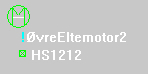
\includegraphics[scale=1.2]{motmod2.jpg}
	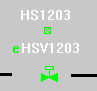
\includegraphics[scale=1.2]{ventmod2.jpg}
	\\Hver motor- og ventil-modul består av en logikkblokk som tar inn signalene og sender signal videre til motorblokken etter slik det er gitt i kravspesifikasjonen.

\subsection{Simulator}
	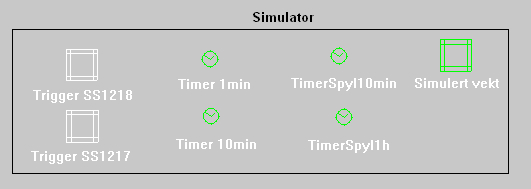
\includegraphics[width=\textwidth]{simulator2.jpg}
	Simuleringspanelet ble lagd for å enklere vise systemets oppførsel. Med det kan man trigge impulsknappen, gi vekt for HS1209A(veiebåndet), og utløse triggeren SS1218 (hastighetsmåleren for haspelen).
